\documentclass[12pt,a4paper]{article}
\usepackage[english,german]{babel}
\usepackage[utf8]{inputenc}
\usepackage{color}
\usepackage{hyperref}
\usepackage{mathtools}
\usepackage{amsmath}
\usepackage{graphicx}
\usepackage{enumitem}

\usepackage{geometry}
\geometry{
  left=3cm,
  right=3cm,
  top=3cm,
  bottom=4cm,
  bindingoffset=5mm
}

\setlength{\parindent}{0em} 
\hypersetup{
    colorlinks=true,
    linktoc=all,
    linkcolor=black,
    urlcolor=black
}

% Hurenkinder und Schusterjungenregel
\clubpenalty = 10000
\widowpenalty = 10000
\displaywidowpenalty = 10000

%Gummi|065|=)
\title{Verhaltensneurogenetik}
\author{}
\date{}

% set title of table of contents
\renewcommand*\contentsname{Inhalt}

% https://www.sharelatex.com/learn
% http://www.math.ubc.ca/~cautis/tools/latexmath.html
% http://www.golatex.de/wiki/Kategorie:Befehlsreferenz
% https://en.wikibooks.org/wiki/LaTeX/Mathematics

\begin{document}

\begin{titlepage}

\maketitle
\thispagestyle{empty}
\end{titlepage}
\newpage

\begin{titlepage}
\tableofcontents
\thispagestyle{empty}
\end{titlepage}
\newpage

\section{Vorlesung 11.05.2016}

\textbf{Flugsimulator}\\
Orientierung im Raum: Fixieren und Bewegung kompensieren\\
Optomotorische Reaktion\\
Fliege folgt der Bewegung des Streifenzylinders\\
Optischer Lobus bei Drosophila\\
Vier optische Neuropile:
\begin{itemize}
	\item Lamina
	\item Medulla
	\item Lobula
	\item Lobulaplatte
\end{itemize}

Ommatidium besteht aus 20 Zellen wobei 8 Photorezeptoren (Retinulazellen R1-R8, welche zweischichtiges Rhadomer bilden) für die Verarbeitung der visuellen Information verantwortlich sind. Adultes Komplexauge besteht aus 800 regelmäßig angeordneten, hexagonalen Einheiten (Ommatidien)\\

omb$^{H31}$-Mutation:
\begin{itemize}
	\item Optomotorische Reaktion im Flug gestört (large field response, not object response)
	\item Optomotorische Reaktion im Lauf weniger gestört
	\item Vermeidung dunkler Objekte
	\item Männliches Balzverhalten gestört
	\item Leichte Störung im Elektroretinogram (ERG)
\end{itemize}

In omb$^{H31}$-Mutation fehlen Riesenneurone der Lobulaplatte
Mutation betrifft das Gen bifid; 40kb-Deletion downstream (regulatorische Region); codiert einen Transkriptionsfaktor\\

\underline{Elementarer Bewegungsdetektor}\\
Wahrnehmung der Luminanzgrenze erst durch Rezeptor A, dann durch Rezeptor B. Je schneller sich Grenze bewegt, je stärkeres Outputsignal (erstmals theoretisch beschrieben von Reichhardt in 1956)\\
Stimulierung des Rezeptor A, dann nach Strecke S Stimulierung des Rezeptor B. Signal A ist verzögert durch Interneuron. Komparator Neuron summiert die Signale\\
Richtung- und Geschwindigkeitsspezifisch\\
Damit beide Richtungen wahrgenommen werden können, Überkreuzschaltung\\
Mutante wird durch Kombination von Gal4-UAS-System und Shi-ts (temperaturempfindliches Protein, 30 $^\circ$C hergestellt -$>$ verhindert Endozytose synaptischer Vesikel\\
Versucht zeigt, dass L1 und L2 Zellen in Lobula Platte als Bewegungsdetekor bei Drosophila fungieren\\

\underline{Augenentwicklung bei Drosophila Melanogaster}\\
Komplexauge besteht aus Ommatidien; jedes einzelne funktioniert als unabhängiger visueller Rezeptor. Zwei Ausrägungen:
\begin{itemize}
	\item Appositionsauge: Ommatidien funktionieren unabhängig (meiste Taginsekten)
	\item Superpositionsauge: Ommatidien kooperieren um ein helleres, überlagenderes Bild auf der Retina zu erzeugen (nachtaktive Insekten)
	\item Beim neuralen Superpositionsauge (schnellfliegende Insekten wie z. B. Drosophila) sind, wie beim Appositionsauge, die Pigmentzellen durchgängig. Im Gegensatz zum Appositionsauge und zum optischen Superpositionsauge gibt es in jedem Ommatidium kein fusioniertes Rhabdom, die zwei mittleren Rhabdomere (7 und 8) liegen hier untereinander. Die sieben einzelnen Rhabdomere sind so angeordnet, dass es ein zentrales Rhabdomer (bestehend aus den beiden Einzelrhabdomeren 7 und 8) und darum jeweils sechs periphere Rhabdomere gibt. Jedes periphere Rhabdomer ist neuronal mit dem zentralen Rhabdomer des gegenüberliegenden Ommatidiums verschaltet, weshalb dieser Augentyp als neuronales Superpositionsauge bezeichnet wird.
\end{itemize}

Ca. 800 Ommatidien mit je 20 Zellen:
\begin{itemize}
	\item 8 Rezeptorzellen
	\item 2 primäre Pigmentzellen
	\item 1 sekundäre Pigmentzelle
	\item 1 tertiäre Pigmentzelle
	\item 4 Kristallkegelzellen
	\item 4 Zellen zur Ausbildung des Haarkomplexes
\end{itemize}

Jede Zelle mit definiertem Platz, d.h. jede Zelle immer mit gleichem Kontakt zu gleichem Satz Nachbarzellen

Das Komplexauge entwickelt sich aus der Augenimaginalscheibe.\\
In der 3. Larve bewegt sich eine synchrone Mitosewelle von posterior nach anterior über die Imaginalscheibe = Start der Differenzierung.\\
Die Mitose ist mit einer Verkürzung der Zellen gekoppelt -> morphogenetische Furche.\\
Räumlicher Abstand zur Furche = Maß des Differenzierungsgrades -> In einer Augenscheibe verschieden weit fortgeschrittene Stadien der Ommatidienentwicklung\\

Wie, in welcher Folge entwickeln sich verschiedene Zelltypen aus einer einschichtigen Epithel? Mitotische Rekombination:
\begin{itemize}
	\item Zellklone in der Augenscheibe, Untersuchung im Grenzbereich
	\item Zellen unterschiedlicher Herkunft werden für ein Ommatidium rekrutiert
	\item Selbst nach der letzten Teilung sind die Zellen noch nicht vollständig determiniert
	\item Induktive, d.h. auf Zell-Zell-Wechselwirkungen, beruhende Entwicklung
\end{itemize}

\underline{Vorteile des Entwicklungsmodells Komplexauge}\\
Identische Untereinheiten in festgelegter Struktur -$>$ jeder Fehler wiederholt sich 800x\\
Mutanten mit defekten Augen / ganz ohne Augen sind unter Laborbedingungen lebensfähig\\
In Näherung zweidimensionales Muster (einschichtiges Epithel)\\

\underline{Festgelegte Reihenfolge der ommatidialen Zelldifferenzierung:}
\begin{enumerate}
	\item R8
	\item R2+R5
	\item R3+R4
	\item R1+R6
	\item R7
	\item Kristallkegelzelle
	\item Primäre Pigmentzelle
	\item Sekundäre und tertiäre Pigmentzelle
\end{enumerate}
R8 = „Organisatorzelle“ (proneurales Potential durch atonal -Expression) laterale Inhibition der Nachbarzellen (sca) (nicht R8)\\

Differenzierung eines Zelltyps verändert die zelluläre Umwelt, wodurch neue Entwicklungsschritte angestoßen werden (induktive Wechselwirkung) $\Rightarrow$
Genetisch bedingte sukzessive Rekrutierung\\

\textbf{Morphogenetische Furche}\\
Inititation:\\
Dpp sezerniertes Molekül, Expression vor Aufreten der Furche am ventralen, dorsalen und posterioren Rand der Augenscheibe. Ektopische Expression von Dpp initiiert Furchenbildung andernorts.\\

Mutante: wingless. Expressioniert ein Dpp-Antagonist. Bei ausreichender Dpp-Überexpression kann wingless-Hemmung überwunden werden, aber es werden weitere Furchen (dorsal und ventral) gebildet\\

\underline{Fortbewegung der Furche:}\\
hedgehog: Segmentpolaritätsgen, sezerniertes Molekül,\\
Expression direkt hinter der Furche\\
initiiert vor der Furche die Dpp-Expression\\
hedghogts-Allele: bei restriktiver Temperatur\\
kommt es zum Stillstand der Furche\\
(Vorteil ts-Allele !!)\\
roughex: Synchronisierung des Zellzyklus in der Furche durch Arretierung in der G1-Phase\\
Posterior der Furche gebildetes Hedehog induziert in den Zellen anterior der Furche die Expressionen von diversen Genen (z.B. ato). Durch Delta-Notch Signal verstärkt ato-Expression und innerhalb der Furche (während der Phase der lateralen Inhibition) erhält ato seine eigene Expression aufrecht. Diese ist jedoch sensibel gegenüber dem jetzt neurogenen Signal von sca/Notch, was schließlich die Reduktion der ato-Expression bewirkt.\\

Die Reichweite der lateralen Inhibition bestimmt die Anzahl und Muster der R8-Zellen.\\

\underline{Sevenless – boss (\textbf{b}rides \textbf{o}f sevenle\textbf{ss}) Mutante}\\
Fehlen der Zelle R7 -$>$ diese werden als letzte Retinulazellen differenziert und detektieren UV-Licht.\\
Sevenless Genprodukt wird in zwei Polypedtidketten gespalten. Beide sind Membrangängig. Sevenless ist Rezeptor für Positionssignal, dass die R7-Vorläuferzelle zur R7 Zelle determiniert.\\

In Augenimaginalscheibe wird boss-Genprodukt nur in R8 gebildet. Heterophile Adhäsion zwischen boss- und sevenless-exprimierenden Zellen. Nur das Boss-Positionierungssignal enthält somit die Information über den richtigen Ort und den richtigen Zeitpunkt der R7-Entwicklung.\\

\textbf{Augenentwicklung Vertebraten – Invertebraten}
Im Gegensatz zum Komplexauge der Insekten, welches aus einer Vielzahl von identischen Einzelaugen besteht, die jeweils au wenigen Zellen aufgebaut sind, ist das Vertebratenauge ein einheitliches Organ von hoher Komplexität. Trotzdem spielen bei der Entwicklung viele der Gene eine Rolle, die bei der Entwicklung des Komplexauges der Insekten von Bedeutung sind. Insbesondere Start- und Endpunkt der Genkaskaden der Augenentwicklung sind in der Evolution konserviert. Bestes Beispiel eyeless / Pax-6 -$>$ Masterkontrollgene für Augenexpression.\\
Pax 6 (bei Maus): heterozygot: kleine Augen, homozygot: letal\\

Ein ganzes Bündel an Proteinen, vorgeschriebener Pfade und Signalkaskaden bilden ein kompliziertes regulatorisches Netzwerk und müssen zusammen funktionieren um das Komplexauge in Drosophila zu bilden.\\

\underline{Das C. Elegans Konnektom}
\begin{itemize}
	\item Einfaches Nervensystem
	\item 302 Neurone
	\item Zellschicksal und neurale Kreise vollständig dokumentiert
\end{itemize}

\underline{Konnektom:}
\begin{itemize}
	\item 302 Neurone
	\item 5000 chemische Synapsen
	\item 600 elektrische Synapsen
	\item 2000 Nerven-Muskel Synapsen
\end{itemize}

\underline{Neuronen können unterteilt werden in:}
\begin{itemize}
	\item Interneuronen
	\item Sensorische Neuronen
	\item Motorneuronen
\end{itemize}

\underline{Kopfneurone:}
\begin{itemize}
	\item Der Nervenring enthält überwiegend sensorische Neurone und fast alle Interneurons
	\item Der Nervenring ist das Gehirn von C. Elegans
\end{itemize}

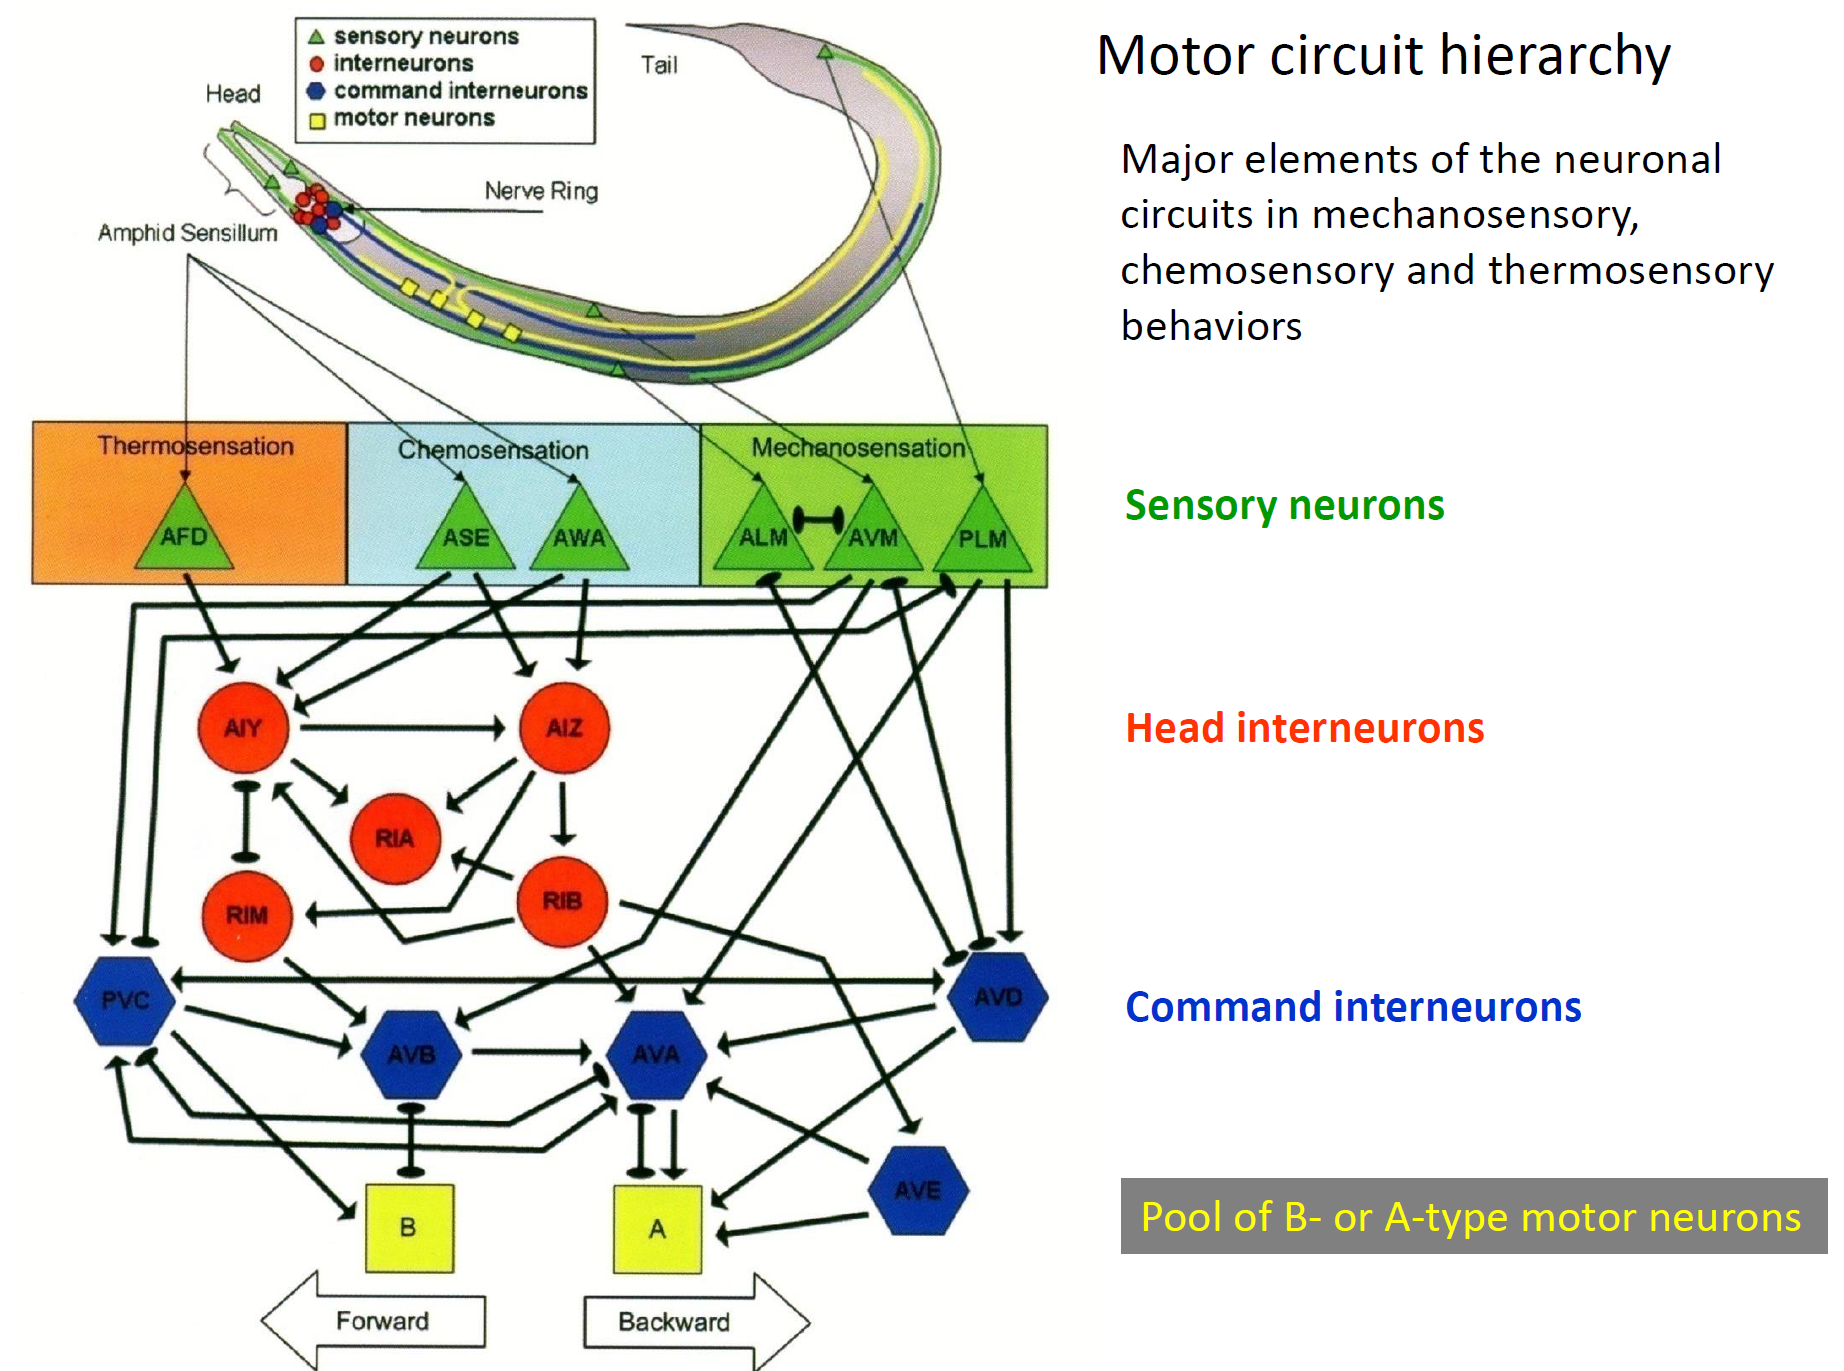
\includegraphics[width=1\textwidth]{lectures/160511/pix/c_elegans_neurones.png}
\\\\
Netzwerk von C. Elegans ist überschaubar. Aber wir wird es gebildet und wie kann man Zugriff darauf erlangen.\\

Axionale Wegfindung in der Entwicklung (beispiel irreC Mutante von Drosophila)
Retinotrope Projektion im Wachstum: Aufrechterhaltung von Nachbarschaftsbeziehungen aus den Augen in den Loben (d.h.: richtige Säule und richtige Schicht)\\

IrreC-Mutation: Fehlerhaftes axonales Wachstum bei R7-, R8-, Laminarmonopolarzellaxonen\\

Struktur-Funktion: Axonales Wachstum, Zellwanderung
\begin{enumerate}
	\item Axonales Wachstum
	\item Zielerkennung
	\item Ausbildung spezifischer Kontakte
\end{enumerate}

Insbesondere bei Vertebraten: Wanderung undifferenzierter Neurone.
Regulative Mechanismen in beiden Fällen ähnlich. Abhängig von Signal-Erkennungs-Mechanismen, nicht zellautonom.\\

Beispiel: Zellen des peripheren Nervensystems (PNS) entstehen in der Neuralleiste und wandern aus, um Ganglien des PNS zu bilden.\\

\end{document}